\subsection{Component Identification in Figure T-2}
\label{T6C08}

\begin{tcolorbox}[colback=gray!10!white,colframe=black!75!black,title=T6C08]
What is component 9 in figure T-2?

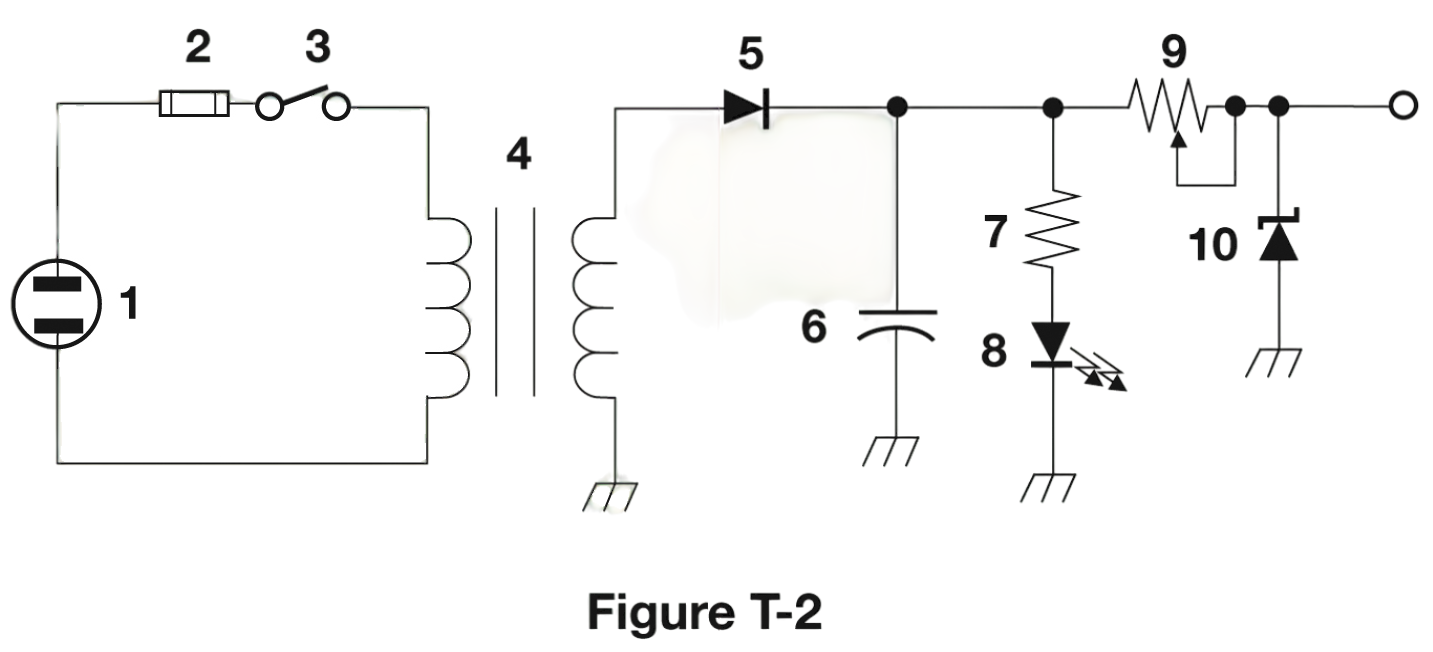
\includegraphics[width=0.5\textwidth]{tech/images/t2.png} 

\begin{enumerate}[label=\Alph*)]
    \item Variable capacitor
    \item Variable inductor
    \item \textbf{Variable resistor}
    \item Variable transformer
\end{enumerate}
\end{tcolorbox}

\subsubsection{Intuitive Explanation}
Imagine you have a volume knob on your stereo. When you turn it, the sound gets louder or softer. That knob is like a variable resistor—it changes how much electricity can flow through it. In figure T-2, component 9 is like that volume knob, but for electricity in a circuit. It’s not a capacitor (which stores energy), an inductor (which resists changes in current), or a transformer (which changes voltage). It’s a variable resistor, which lets you adjust the flow of electricity.

\subsubsection{Advanced Explanation}
In electronic circuits, a variable resistor, also known as a potentiometer or rheostat, is a component that allows the resistance in a circuit to be adjusted manually. This adjustment can control the current flow or voltage levels within the circuit. Mathematically, the resistance \( R \) of a variable resistor can be expressed as:

\[ R = \rho \frac{L}{A} \]

where \( \rho \) is the resistivity of the material, \( L \) is the length of the resistive element, and \( A \) is the cross-sectional area. By changing \( L \) or \( A \), the resistance can be varied. In figure T-2, component 9 is identified as a variable resistor because it is designed to allow such adjustments, unlike capacitors, inductors, or transformers, which have different functions and properties.

% Prompt for diagram: Generate a diagram showing a simple circuit with a variable resistor labeled as component 9, along with other components for context.